\documentclass[11pt,letterpaper]{article}
\input{glyphtounicode}
\pdfgentounicode=1
\usepackage[utf8]{inputenc}
\usepackage[T1]{fontenc}
\usepackage{lmodern}
\usepackage[spanish,es-noindentfirst,es-tabla]{babel}
\decimalpoint
\usepackage[margin=2.5cm]{geometry}
\usepackage{graphicx}
\usepackage{booktabs}
\usepackage{array}
\usepackage{multirow}
\usepackage{siunitx}
\sisetup{output-decimal-marker={.}, group-digits=false, detect-weight=true, table-number-alignment=center}
\usepackage{amsmath,amssymb}
\usepackage{listings}
\renewcommand{\lstlistingname}{Código}
\usepackage{xcolor}
\usepackage{tikz}
\usetikzlibrary{positioning,arrows.meta,shapes.geometric}
\usepackage{fancyhdr}
\usepackage{titlesec}
\usepackage{caption}
\usepackage[section]{placeins}
\usepackage[hidelinks]{hyperref}
\graphicspath{{figuras/}}
\renewcommand{\topfraction}{0.92}
\renewcommand{\bottomfraction}{0.85}
\renewcommand{\textfraction}{0.06}
\renewcommand{\floatpagefraction}{0.80}
\setcounter{topnumber}{3}
\setcounter{totalnumber}{5}
\captionsetup{font=small,labelfont=bf}

\lstdefinestyle{codigo}{
    language=Python,
    basicstyle=\ttfamily\footnotesize,
    keywordstyle=\color{blue!60!black}\bfseries,
    commentstyle=\color{gray},
    stringstyle=\color{orange!70!black},
    numbers=left,
    numberstyle=\tiny\color{gray},
    frame=single,
    breaklines=true,
    showstringspaces=false,
    tabsize=4,
    backgroundcolor=\color{gray!5},
    extendedchars=true,
    columns=fullflexible,
    keepspaces=true,
    literate={á}{{\'a}}1 {é}{{\'e}}1 {í}{{\'i}}1 {ó}{{\'o}}1 {ú}{{\'u}}1
             {Á}{{\'A}}1 {É}{{\'E}}1 {Í}{{\'I}}1 {Ó}{{\'O}}1 {Ú}{{\'U}}1
             {ñ}{{\~n}}1 {Ñ}{{\~N}}1 {¿}{{?`}}1 {¡}{{!`}}1 {±}{{$\pm$}}1
}
\lstset{style=codigo}

\pagestyle{fancy}
\fancyhf{}
\rhead{Inteligencia Computacional Aplicada}
\cfoot{\thepage}
\renewcommand{\headrulewidth}{0.4pt}
\titleformat{\section}{\normalfont\Large\bfseries}{\thesection.}{0.5em}{}
\titleformat{\subsection}{\normalfont\large\bfseries}{\thesubsection}{0.5em}{}

\newcommand{\nombreEstudiante}{Sergio Santiago Duarte Rojas}
\newcommand{\codigoEstudiante}{20261595002}
\newcommand{\nombreDocente}{Cesar Andrey Perdomo Charry}
\newcommand{\nombreAsignatura}{Inteligencia Computacional Aplicada}

% Diagramas de arquitectura
\definecolor{cEntrada}{RGB}{230,230,230}
\definecolor{cConv}{RGB}{204,224,240}
\definecolor{cPool}{RGB}{255,228,204}
\definecolor{cDensa}{RGB}{212,236,222}
\definecolor{cReg}{RGB}{236,220,240}
\tikzset{
    capa/.style={draw=black!60, rounded corners=2pt, minimum height=1.05cm, text width=1.95cm, align=center, font=\footnotesize, inner sep=2pt},
    tensor/.style={font=\scriptsize, text=black!70},
    flecha/.style={-{Latex[length=1.6mm]}, black!70},
}
\definecolor{cDifuso}{RGB}{255,240,200}

\input{cifras}
\hypersetup{pdftitle={Actividad 4. Clasificación difusa del movimiento de un robot}, pdfauthor={Sergio Santiago Duarte Rojas}}
\lhead{Actividad 4, taller adicional}

\begin{document}

\begin{titlepage}
    \centering
    \vspace*{2cm}
    {\LARGE \bfseries Actividad 4. Taller de lógica difusa (adicional)\\[4pt] Clasificación difusa del movimiento de un robot que sigue la pared\par}
    \vspace{0.5cm}
    {\large Informe\par}
    \vspace{2cm}
    \begin{tabular}{ll}
        \textbf{Asignatura:} & \nombreAsignatura \\
        \textbf{Docente:}    & \nombreDocente \\
        \textbf{Estudiante:} & \nombreEstudiante \\
        \textbf{Código:}     & \codigoEstudiante \\
        \textbf{Fecha:}      & \today \\
    \end{tabular}
    \vfill
    Universidad Distrital Francisco José de Caldas
\end{titlepage}

\tableofcontents
\newpage

\section{Introducción}

El taller pide construir dos modelos de lógica difusa que clasifiquen la acción de un robot a partir de sus sensores, uno con cuatro entradas y otro con dos. Las funciones de pertenencia de cada entrada deben salir del análisis de datos, es decir de los histogramas, los histogramas por clase y las nubes de puntos, y el número de reglas, que es el producto del número de etiquetas de cada variable, no puede pasar de 100.

Los histogramas por clase muestran que las cuatro acciones quedan separadas por completo con tres umbrales sobre dos distancias, la frontal y la izquierda. Las distancias derecha y trasera aportan información por sí solas, pero no agregan nada una vez conocidas las otras dos. Con esos umbrales como cruces de las funciones de pertenencia, el modelo de dos sensores tiene \reglasDos{} reglas y el de cuatro \reglasCuatro, y los dos clasifican bien los \nTe{} registros de prueba. Con etiquetas uniformes ninguna variante pasa de \uniMejor~\% dentro del límite de reglas. El trabajo parte de la experiencia del taller propuesto y se hizo en Python con las funciones del cuaderno resuelto de la clase. El cuaderno entregado se ejecutó completo con las dieciocho verificaciones en \texttt{[OK]}. Junto con el informe se entregan los datos, los grupos de entrenamiento y de prueba de cada partición y los dos modelos, que permiten repetir el experimento (Anexo~\ref{anexo:archivos}).

\section{Marco teórico (resumen)}

\subsection{Etiquetas trapezoidales}

Una etiqueta como «cerca» es un conjunto difuso que asigna a cada distancia un grado entre 0 y 1 (Zadeh, 1965). La trapezoidal $\mathrm{trapmf}(x;[a\ b\ c\ d])$ vale 1 entre $b$ y $c$, sube linealmente de $a$ a $b$ y baja de $c$ a $d$ (Ross, 2010). Dos trapecios vecinos que se cruzan en 0.5 en un valor $u$, con una transición de semiancho $\delta$, describen una frontera difusa. Lejos de $u$ el dato pertenece del todo a una etiqueta y dentro de la franja $[u-\delta, u+\delta]$ pertenece en parte a las dos, con grados que suman uno.

\subsection{Base de reglas en rejilla}

Si cada variable tiene $n_j$ etiquetas, la rejilla completa tiene $\prod_j n_j$ reglas, una por cada combinación de etiquetas. Con 3 etiquetas en 4 variables son $3^4=81$, y con 4 etiquetas ya serían 256. Por eso el límite de 100 reglas obliga a decidir con los datos cuántas etiquetas merece cada variable. La fuerza de una regla ante un registro combina los grados de sus antecedentes con una t-norma, la operación que representa la Y, aquí el producto. El consecuente de cada regla se aprende del entrenamiento como en el método de Ishibuchi, Nozaki y Tanaka (1992). Cada regla toma la acción cuyos registros la activan con mayor fuerza total. La certeza que se informa es la fracción de esa fuerza que aporta la acción elegida, una versión simplificada del grado de certeza de Ishibuchi et al. que aquí no interviene en la clasificación. El cuaderno resuelto usa en cambio la idea de Wang y Mendel (1992), que da a cada regla la clase del registro de mayor grado.

\subsection{Clasificación, salida continua y medidas}

Para clasificar un registro nuevo se calcula la fuerza de todas las reglas y gana la más fuerte, como en el clasificador del cuaderno resuelto. Un Sugeno de orden cero usa las mismas reglas de otra forma. Cada regla propone una constante, aquí un giro, y la salida es el promedio de esas constantes ponderado por la fuerza de cada regla (Takagi y Sugeno, 1985). Además de la exactitud se informa la exactitud balanceada, el promedio del acierto de cada clase, porque una de las cuatro acciones es solo el 6~\% de los registros.

\section{Metodología}

\subsection{Punto de partida, el taller propuesto}

El taller propuesto aplicó a Wine el clasificador de Wang y Mendel con etiquetas uniformes. Con tres etiquetas obtuvo 92.6~\% en prueba con 31 reglas, y con las cuatro etiquetas que eligió la validación cruzada 88.9~\% con 43. De ese taller se toman cinco decisiones. Todo lo que define el modelo (cortes, etiquetas, consecuentes y elección entre modelos) se calcula solo con el entrenamiento, y la prueba se mide una vez al final. La t-norma es el producto, porque allí el mínimo y el producto dieron las mismas 54 predicciones, ya que con la regla más fuerte gana la celda propia de cada registro. Con tres etiquetas, tres de los cuatro errores de aquel taller caían en celdas dominadas por otro cultivar, uno en la única regla cuyo consecuente, tomado del registro de mayor grado, no seguía a la mayoría, y con más etiquetas aparecían celdas casi vacías. Por eso aquí el consecuente sale de la suma de fuerzas de todos los registros y se revisa el soporte de cada regla. Como allí, el modelo se compara con un árbol de decisión con el mismo límite de hojas. Por último, las reglas se prueban también como Sugeno de orden cero, el tipo de sistema que allí se ajustó con ANFIS. Lo que aquel taller no resolvió, dónde poner las etiquetas cuando la partición uniforme no sirve, es lo que este resuelve con los histogramas por clase.

\subsection{Datos}

Los datos vienen de un robot SCITOS G5 que recorrió cuatro veces una sala siguiendo la pared en el sentido de las agujas del reloj, con 24 sensores de ultrasonido alrededor del cuerpo. Según sus autores, la acción de cada registro la asignó un clasificador heurístico de reglas SI ENTONCES (Freire et al., 2009a). Los dos archivos del taller traen distancias simplificadas, la menor lectura de los sensores de cada arco de 60 grados (Freire et al., 2009b). \texttt{sensor\_readings\_4.csv} tiene las distancias frontal, izquierda, derecha y trasera, y \texttt{sensor\_readings\_2.csv} solo las dos primeras. El cuaderno comprueba que el segundo archivo es el primero sin las dos últimas columnas, registro por registro. La Tabla~\ref{tab:clases} muestra las cuatro acciones, ordenadas de derecha a izquierda como un volante. En los \nReg{} registros las lecturas se saturan en 5.0, valor que aparece \satD{} veces en la distancia trasera, \satA{} en la frontal, \satC{} en la derecha y \satB{} en la izquierda.

\begin{table}[!htb]
    \centering
    \caption{Acciones del robot en los \nReg{} registros y en la partición de prueba}
    \label{tab:clases}
    \footnotesize
    \begin{tabular}{l l S[table-format=4.0] S[table-format=2.1] S[table-format=3.0]}
        \toprule
        \textbf{Acción} & \textbf{Etiqueta en el archivo} & {\textbf{Registros}} & {\textbf{\%}} & {\textbf{En prueba}} \\
        \midrule
        Giro fuerte a la derecha & Sharp-Right-Turn & 2097 & \pctA & \cuentaTeA \\
        Giro suave a la derecha & Slight-Right-Turn & 826 & \pctB & \cuentaTeB \\
        Avanzar & Move-Forward & 2205 & \pctC & \cuentaTeC \\
        Giro suave a la izquierda & Slight-Left-Turn & 328 & \pctD & \cuentaTeD \\
        \bottomrule
    \end{tabular}
\end{table}

\subsection{Particiones}

Los registros se parten de forma estratificada en 70~\% para entrenar y 30~\% para probar, \nTr{} y \nTe, con semilla 42 y la misma partición para los dos modelos. Todo el análisis de datos, los umbrales, las etiquetas, los consecuentes y la elección entre modelos usan solo el entrenamiento, y la prueba se mide al final. Los registros vienen de un recorrido continuo, y entre dos registros seguidos la mediana del cambio va de \cambioMin{} a \cambioMax{} según el sensor, mientras que la acción cambia solo en el \cambioAccion~\% de los pares. La partición aleatoria pone entonces en prueba registros muy parecidos a otros de entrenamiento. Por eso se repite el diseño completo con una partición temporal, el primer 70~\% del recorrido para entrenar y el último 30~\% para probar.

\subsection{Diseño de las funciones de pertenencia}

En las variables cuyas clases no se solapan, cada umbral que muestran los histogramas por clase se fija como el punto medio entre el mayor valor de la clase que queda debajo y el menor de la que queda encima, en el entrenamiento. Ese punto medio solo vale porque las clases no se tocan, algo que el cuaderno verifica. En las variables cuyas clases se solapan, el corte es el valor que mejor separa las acciones con esa variable sola, el que elige un árbol de decisión de un nivel. Alrededor de cada corte las etiquetas vecinas son trapecios que se cruzan en 0.5, con semiancho $\delta=\semiancho$ fijado a mano. Las distancias derecha y trasera reciben dos etiquetas cada una, el mínimo para que intervengan en las reglas, lo que deja la rejilla del modelo de cuatro entradas en $2\times3\times2\times2=24$ reglas. La Figura~\ref{fig:flujo} resume el proceso.

\begin{figure}[!htb]
    \centering
    \begin{tikzpicture}[node distance=0.32cm]
        \node[capa, fill=cEntrada] (d) {Distancias\\4 o 2 sensores};
        \node[capa, fill=cConv, right=of d] (a) {Histogramas\\y nubes};
        \node[capa, fill=cConv, right=of a] (u) {Cortes por\\clase};
        \node[capa, fill=cDifuso, right=of u] (t) {Trapecios\\$\delta=\semiancho$};
        \node[capa, fill=cDifuso, right=of t] (r) {Rejilla\\de reglas};
        \node[capa, fill=cDifuso, below=0.9cm of r] (c) {Consecuente\\por fuerza};
        \node[capa, fill=cDensa, left=of c] (g) {Regla más\\fuerte};
        \node[capa, fill=cPool, left=of g] (e) {Acción del\\robot};
        \draw[flecha] (d) -- (a); \draw[flecha] (a) -- (u); \draw[flecha] (u) -- (t); \draw[flecha] (t) -- (r);
        \draw[flecha] (r) -- (c); \draw[flecha] (c) -- (g); \draw[flecha] (g) -- (e);
        \node[tensor, above=0.02cm of a] {solo entrenamiento};
        \node[tensor, above=0.02cm of r] {máximo 100};
        \node[tensor, below=0.02cm of c] {suma de fuerzas};
    \end{tikzpicture}
    \caption{Diseño de los dos modelos. Los bloques amarillos son la parte difusa}
    \label{fig:flujo}
\end{figure}

\subsection{Comparaciones}

Antes de mirar la prueba, los dos modelos se comparan con validación cruzada de cinco particiones en el entrenamiento. En prueba se comparan con un árbol de decisión al que se le permiten tantas hojas como reglas tiene el modelo difuso. Para separar el efecto de dónde se ponen las etiquetas del efecto del método de reglas, se prueban además cuatro variantes con etiquetas uniformes dentro del límite de 100 reglas. Las etiquetas pueden repartirse entre el mínimo y el máximo del entrenamiento, como en el cuaderno resuelto, o con igual frecuencia, según los cuantiles del entrenamiento. El consecuente puede salir del registro de mayor grado o de la suma de fuerzas. En cada variante el número de etiquetas se elige con validación cruzada en el entrenamiento. Por último se mide cuánto depende el resultado de la posición de cada umbral, del semiancho $\delta$ y de un ruido gaussiano en las lecturas, y se evalúan las seis reglas como un Sugeno de orden cero.

\section{Resultados}

\subsection{Análisis de datos}

La Figura~\ref{fig:hist} muestra los histogramas de cada distancia en escala logarítmica. Las cuatro tienen la mayor parte de las lecturas por debajo de 3.5. La izquierda, la derecha y la trasera tienen además una cola de lecturas aisladas hasta 5.0, y la frontal solo un grupo de lecturas en 5.0. La Figura~\ref{fig:histclase} separa los histogramas por acción y la Figura~\ref{fig:nubes} muestra las nubes de puntos.

\begin{figure}[!htb]
    \centering
    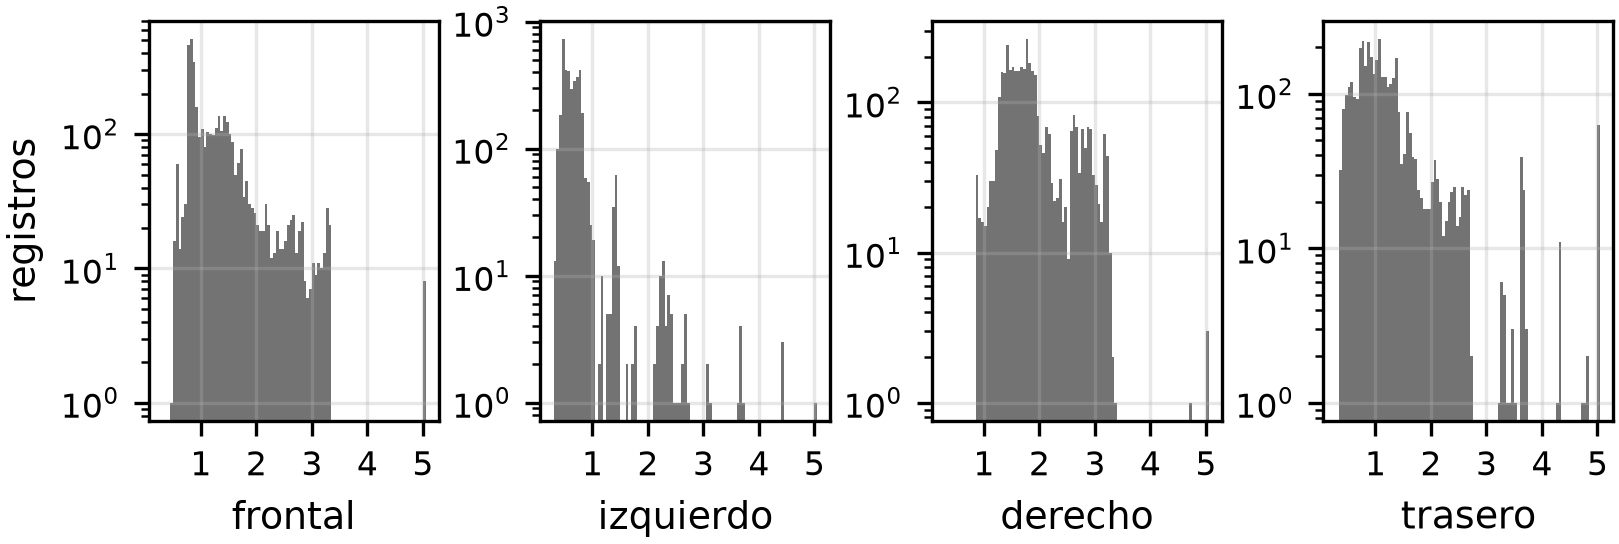
\includegraphics[width=15.5cm]{fig01_histogramas.png}
    \caption{Histograma de cada distancia en el entrenamiento, con el eje vertical en escala logarítmica}
    \label{fig:hist}
\end{figure}

\begin{figure}[!htb]
    \centering
    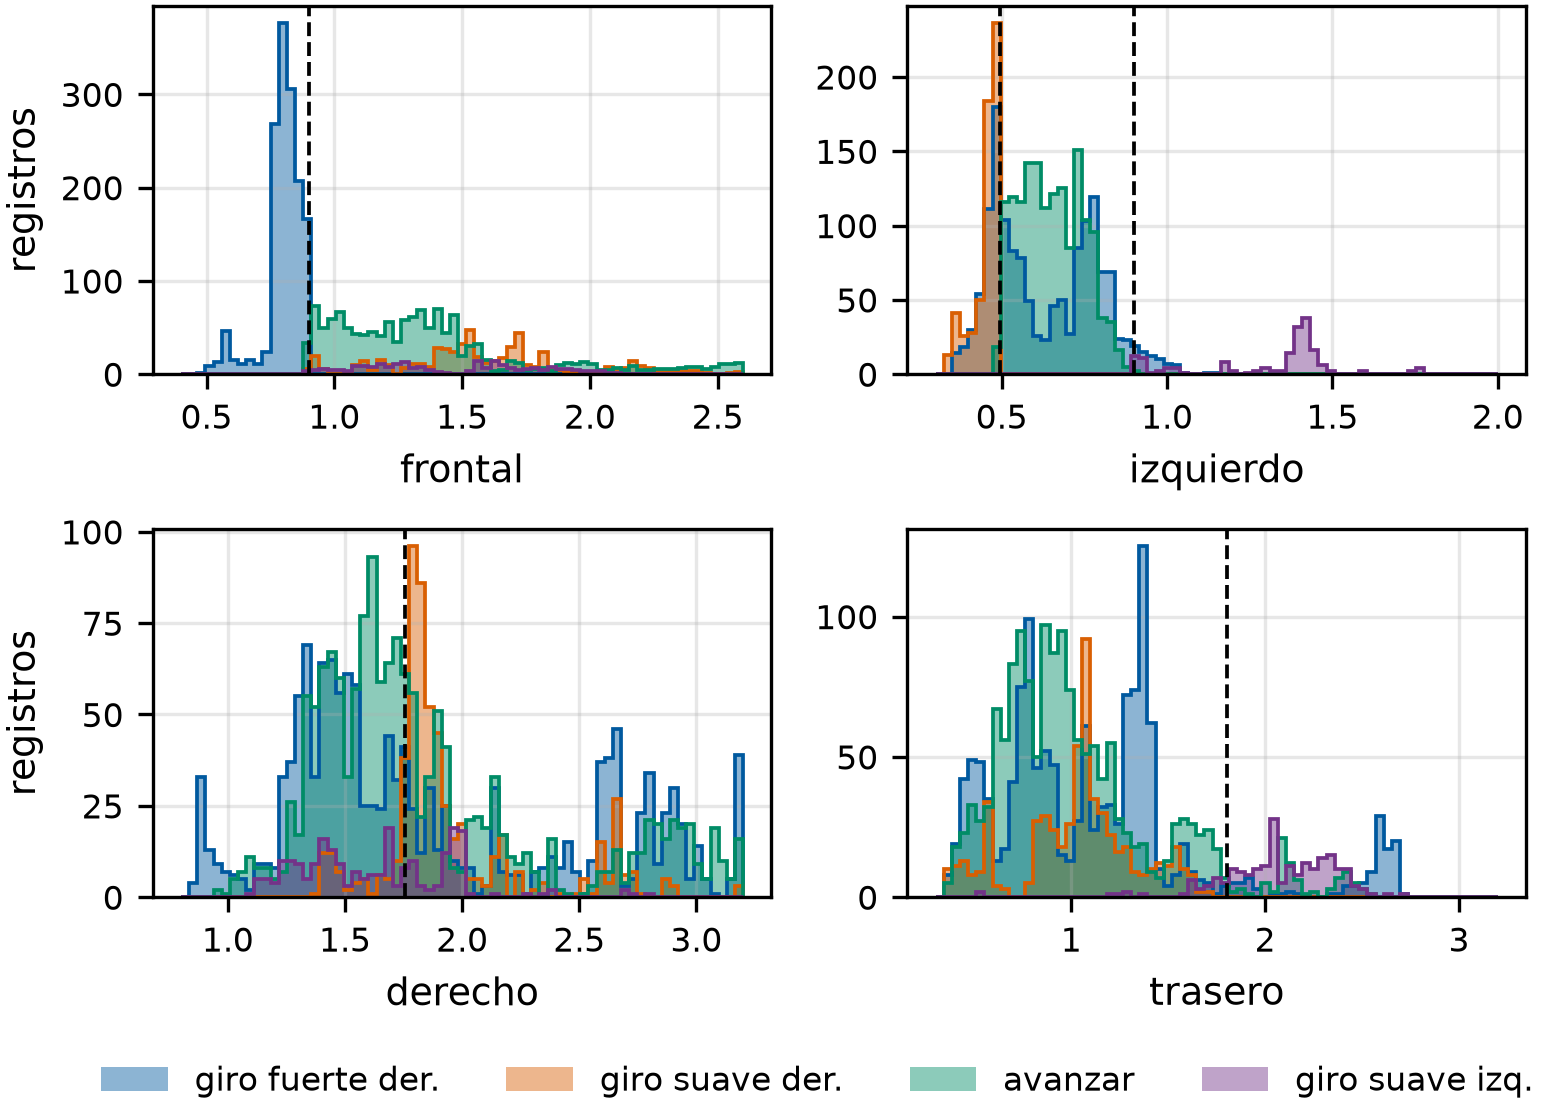
\includegraphics[width=15cm]{fig02_histogramas_clase.png}
    \caption{Histogramas por acción en el entrenamiento, con cada eje vertical en su propia escala. Las líneas discontinuas marcan los cortes elegidos. Los ejes horizontales se recortan a la zona más densa y dejan fuera \fueraHist{} lecturas en total}
    \label{fig:histclase}
\end{figure}

\begin{figure}[!htb]
    \centering
    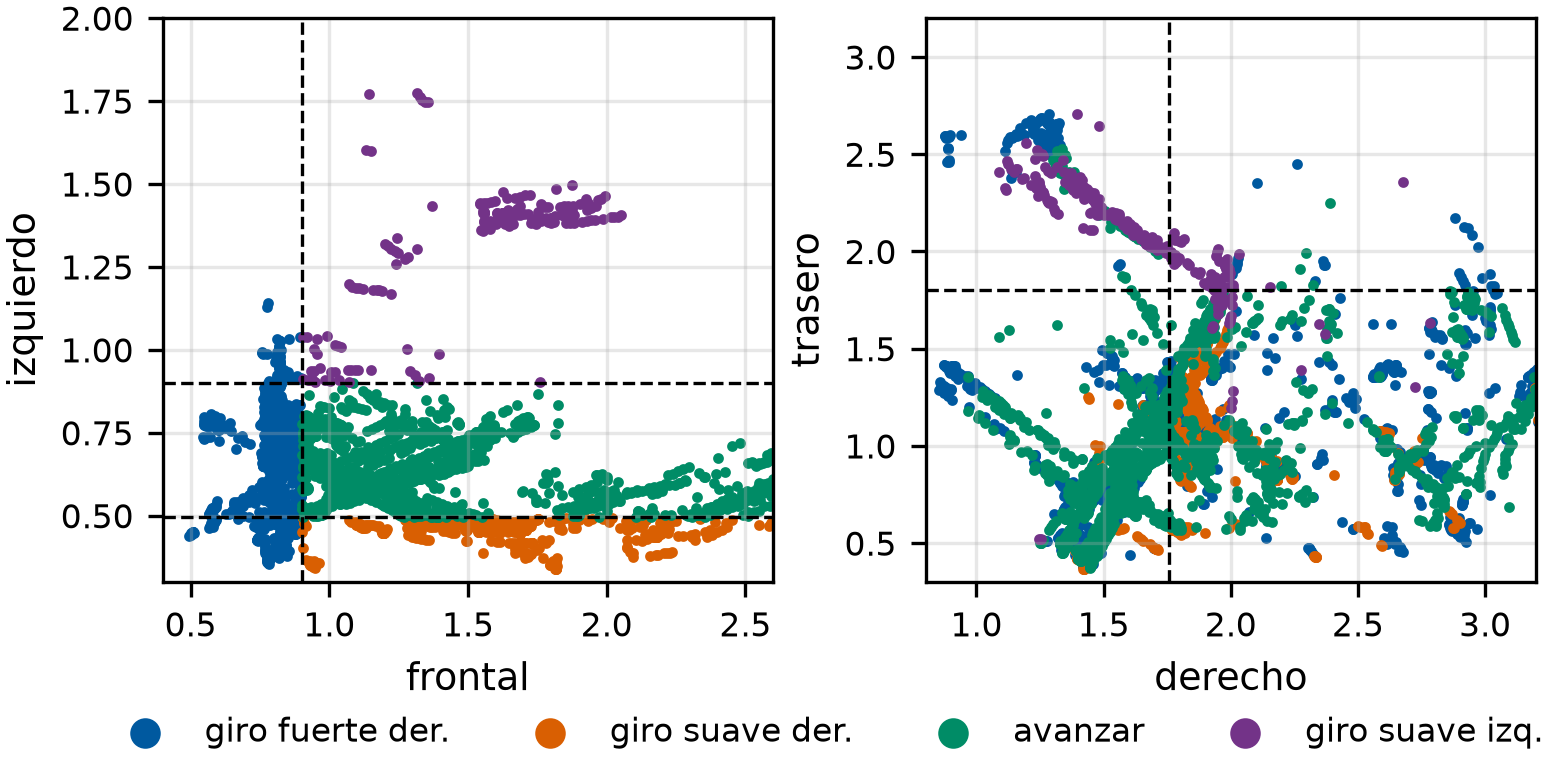
\includegraphics[width=15cm]{fig03_nubes.png}
    \caption{Nubes de puntos del entrenamiento con los cortes elegidos. Izquierda, frontal frente a izquierda. Derecha, derecha frente a trasera. Los ejes se recortan a la zona más densa y dejan fuera \fueraNubeA{} registros en el panel izquierdo y \fueraNubeB{} en el derecho}
    \label{fig:nubes}
\end{figure}

La Tabla~\ref{tab:rangos} da el rango de las dos primeras distancias por acción. El giro fuerte a la derecha ocurre siempre con la distancia frontal hasta 0.900 y las otras tres acciones empiezan en 0.901. Entre esas tres, la distancia izquierda forma franjas que no se tocan, giro suave a la derecha hasta 0.494, avanzar entre 0.495 y 0.900 y giro suave a la izquierda desde 0.902. En las distancias derecha y trasera los rangos de todas las acciones se superponen (Tabla~\ref{tab:rangosdt}). Aun así separan en parte algunas acciones. Por encima del corte de la trasera queda el \trasIzq~\% de los registros de giro suave a la izquierda y como mucho el \trasOtrasMax~\% de las demás acciones. Por encima del corte de la derecha queda el \derSuave~\% de los de giro suave a la derecha y como mucho el \derOtrasMax~\% de las demás. Un árbol sin límite entrenado solo con esas dos distancias acierta el \accSoloDT~\% de la prueba aleatoria, frente al \mayoritaria~\% de la clase mayoritaria, pero con \hojasSoloDT{} hojas que memorizan tramos del recorrido. Con la partición temporal acierta el \accSoloDTt~\%, todavía por encima del \mayT~\% de la clase mayoritaria.

\begin{table}[!htb]
    \centering
    \caption{Valores mínimo y máximo de las distancias frontal e izquierda por acción, en el entrenamiento}
    \label{tab:rangos}
    \footnotesize
    \begin{tabular}{l S[table-format=1.3] S[table-format=1.3] S[table-format=1.3] S[table-format=1.3]}
        \toprule
         & \multicolumn{2}{c}{\textbf{Frontal}} & \multicolumn{2}{c}{\textbf{Izquierda}} \\
        \cmidrule(lr){2-3} \cmidrule(lr){4-5}
        \textbf{Acción} & {\textbf{Mínimo}} & {\textbf{Máximo}} & {\textbf{Mínimo}} & {\textbf{Máximo}} \\
        \midrule
\filasRangos
        \bottomrule
    \end{tabular}
\end{table}

\begin{table}[!htb]
    \centering
    \caption{Mínimo, mediana y máximo de las distancias derecha y trasera por acción, y porcentaje de registros por encima de cada corte, en el entrenamiento}
    \label{tab:rangosdt}
    \scriptsize
    \setlength{\tabcolsep}{4pt}
    \begin{tabular}{l S[table-format=1.2] S[table-format=1.2] S[table-format=1.2] S[table-format=1.2] S[table-format=1.2] S[table-format=1.2] S[table-format=2.1] S[table-format=2.1]}
        \toprule
         & \multicolumn{3}{c}{\textbf{Derecha}} & \multicolumn{3}{c}{\textbf{Trasera}} & \multicolumn{2}{c}{\textbf{\% sobre el corte}} \\
        \cmidrule(lr){2-4} \cmidrule(lr){5-7} \cmidrule(lr){8-9}
        \textbf{Acción} & {\textbf{Mín.}} & {\textbf{Mediana}} & {\textbf{Máx.}} & {\textbf{Mín.}} & {\textbf{Mediana}} & {\textbf{Máx.}} & {\textbf{Derecha}} & {\textbf{Trasera}} \\
        \midrule
\filasRangosDT
        \bottomrule
    \end{tabular}
\end{table}

\subsection{Funciones de pertenencia}

Los umbrales quedaron en \uFrontal{} para la distancia frontal y en \uIzqBajo{} y \uIzqAlto{} para la izquierda, los puntos medios entre los límites de clase de la Tabla~\ref{tab:rangos}. Los cortes del árbol de un nivel son \uDerecho{} para la derecha y \uTrasero{} para la trasera. La Tabla~\ref{tab:mf} da los parámetros y la Figura~\ref{fig:mf} dibuja las etiquetas sobre el histograma de cada variable. En los extremos los trapecios se extienden fuera del rango de las lecturas, hasta $-1$ y 6, para que las etiquetas de los extremos cubran cualquier lectura, desde la más baja hasta la saturación en 5.0.

\begin{table}[!htb]
    \centering
    \caption{Etiquetas de cada variable, todas trapezoidales con parámetros $[a\ b\ c\ d]$}
    \label{tab:mf}
    \footnotesize
    \begin{tabular}{l l l}
        \toprule
        \textbf{Variable} & \textbf{Etiqueta} & \textbf{Parámetros} \\
        \midrule
\filasMF
        \bottomrule
    \end{tabular}
\end{table}

\begin{figure}[!htb]
    \centering
    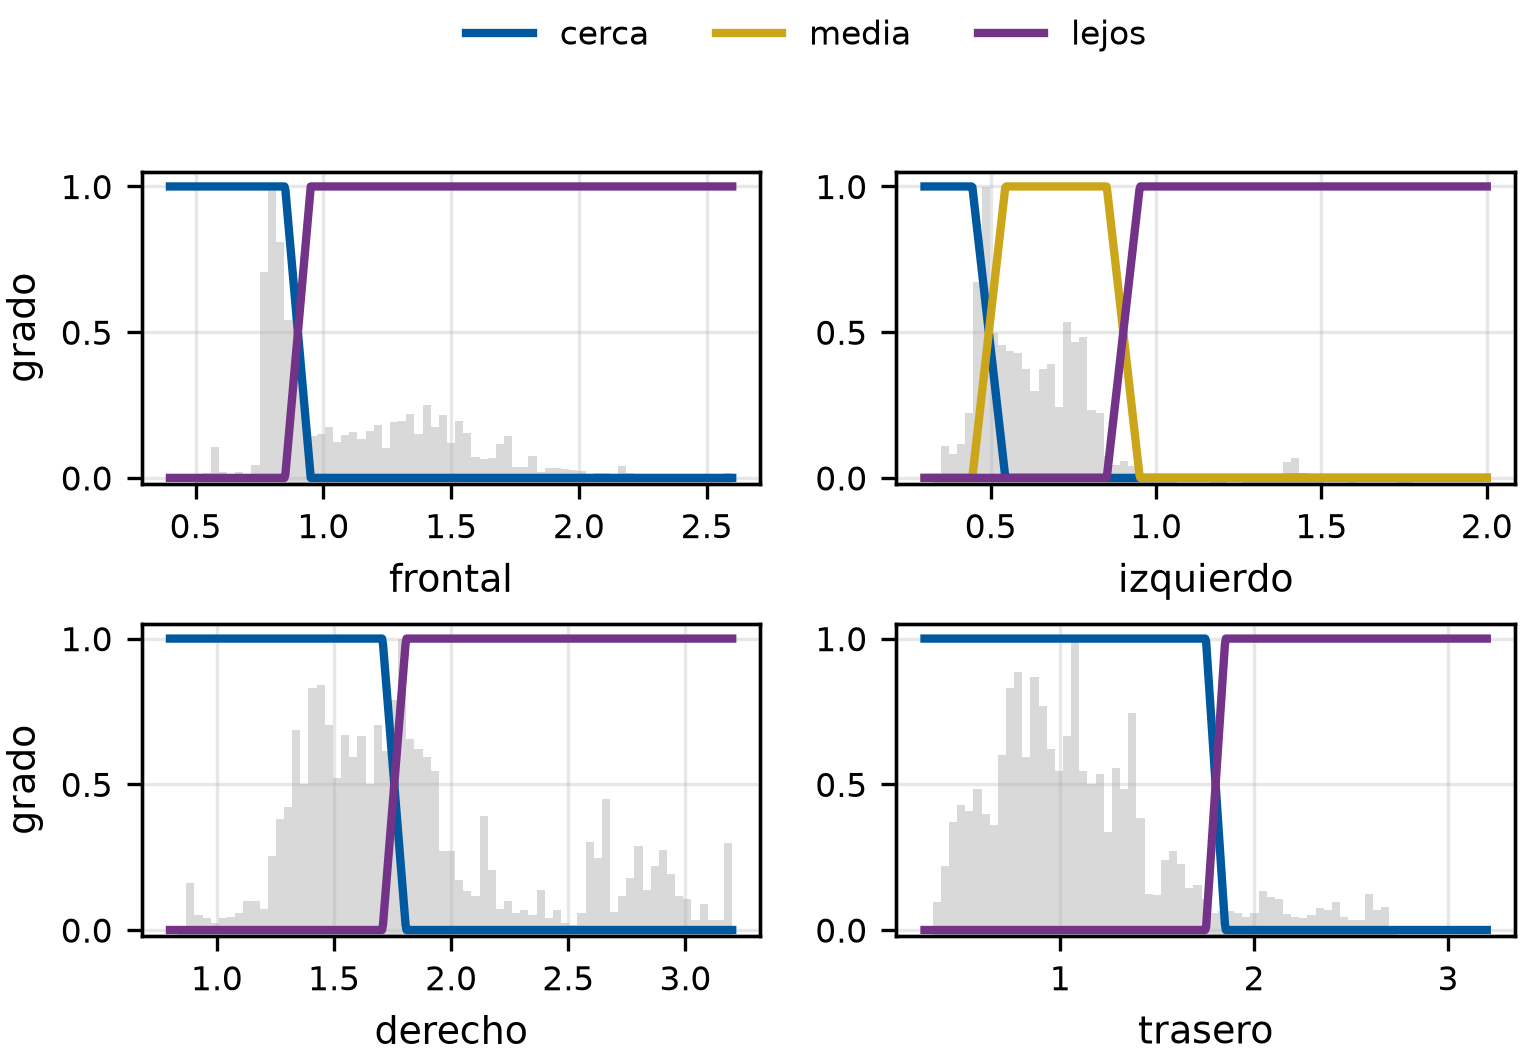
\includegraphics[width=15cm]{fig04_pertenencia.png}
    \caption{Etiquetas de cada variable sobre su histograma de entrenamiento, en gris}
    \label{fig:mf}
\end{figure}

\subsection{Reglas}

La rejilla de dos entradas tiene $2\times3=6$ reglas y la de cuatro $2\times3\times2\times2=24$, las dos por debajo del límite de 100, y ninguna tiene soporte nulo en el entrenamiento. La Tabla~\ref{tab:reglas} muestra las seis reglas del modelo de dos sensores. El soporte es la suma de la fuerza con que los registros de entrenamiento activan la regla, la certeza es la fracción de ese soporte que viene de la acción elegida, y la última columna cuenta en cuántos registros de prueba la regla fue la ganadora. Las 24 reglas del modelo de cuatro sensores están en el Anexo~\ref{anexo:reglas}. En \nDistintas{} de ellas la acción aprendida no coincide con la que dictan solo la distancia frontal y la izquierda. Son \distReglas. Sus soportes son \distSoportes, no ganan en ningún registro de prueba y su acción sale de lecturas que caen en franjas de transición de otras reglas.

\begin{table}[!htb]
    \centering
    \caption{Las seis reglas del modelo de dos sensores, ordenadas por soporte en el entrenamiento}
    \label{tab:reglas}
    \footnotesize
    \begin{tabular}{c l l l S[table-format=4.1] S[table-format=1.3] S[table-format=3.0]}
        \toprule
        \textbf{Regla} & \textbf{Si frontal es} & \textbf{y izquierda es} & \textbf{Entonces} & {\textbf{Soporte}} & {\textbf{Certeza}} & {\textbf{Gana}} \\
        \midrule
\filasReglasDos
        \bottomrule
    \end{tabular}
\end{table}

\subsection{Evaluación en prueba}

En la validación cruzada del entrenamiento los dos modelos aciertan el \cvDos~\%. La Tabla~\ref{tab:resultados} resume la prueba. Los dos modelos difusos aciertan los \nTe{} registros, con exactitud y exactitud balanceada del 100~\%, y la matriz de confusión es diagonal (Tabla~\ref{tab:confusion}). Los dos modelos guardados en disco y vueltos a cargar reproducen esas predicciones sobre los archivos de prueba. El árbol de decisión, con permiso para \reglasCuatro{} hojas, solo usa \hojasCuatro, corta en \uFrontal, \uIzqBajo{} y \uIzqAlto{} y también acierta todo. La regla nítida de tres umbrales, frontal hasta \uFrontal{} y luego izquierda hasta \uIzqBajo{} y hasta \uIzqAlto, acierta los \aciertosNitida{} registros del archivo. La Figura~\ref{fig:mapa} muestra las regiones que asigna el modelo de dos sensores, con las franjas de transición sombreadas y los registros de prueba encima.

\begin{table}[!htb]
    \centering
    \caption{Exactitud en prueba, en porcentaje, sobre \nTe{} registros}
    \label{tab:resultados}
    \footnotesize
    \begin{tabular}{l l S[table-format=2.0] S[table-format=3.1] S[table-format=3.1]}
        \toprule
        \textbf{Entradas} & \textbf{Modelo} & {\textbf{Reglas u hojas}} & {\textbf{Exactitud}} & {\textbf{Balanceada}} \\
        \midrule
        \multirow{2}{*}{4 sensores} & Difuso, cortes del análisis & \reglasCuatro & \accCuatro & \balCuatro \\
                                    & Árbol de decisión & \hojasCuatro & \arbolCuatro & 100.0 \\
        \midrule
        \multirow{2}{*}{2 sensores} & Difuso, cortes del análisis & \reglasDos & \accDos & \balDos \\
                                    & Árbol de decisión & \hojasDos & \arbolDos & 100.0 \\
        \bottomrule
    \end{tabular}
\end{table}

\begin{table}[!htb]
    \centering
    \caption{Matriz de confusión en prueba, igual para los dos modelos difusos. Filas, acción real. Columnas, acción predicha}
    \label{tab:confusion}
    \footnotesize
    \begin{tabular}{l S[table-format=3.0] S[table-format=3.0] S[table-format=3.0] S[table-format=2.0]}
        \toprule
         & {\textbf{Giro fuerte der.}} & {\textbf{Giro suave der.}} & {\textbf{Avanzar}} & {\textbf{Giro suave izq.}} \\
        \midrule
        Giro fuerte a la derecha & \cuentaTeA & 0 & 0 & 0 \\
        Giro suave a la derecha & 0 & \cuentaTeB & 0 & 0 \\
        Avanzar & 0 & 0 & \cuentaTeC & 0 \\
        Giro suave a la izquierda & 0 & 0 & 0 & \cuentaTeD \\
        \bottomrule
    \end{tabular}
\end{table}

\begin{figure}[!htb]
    \centering
    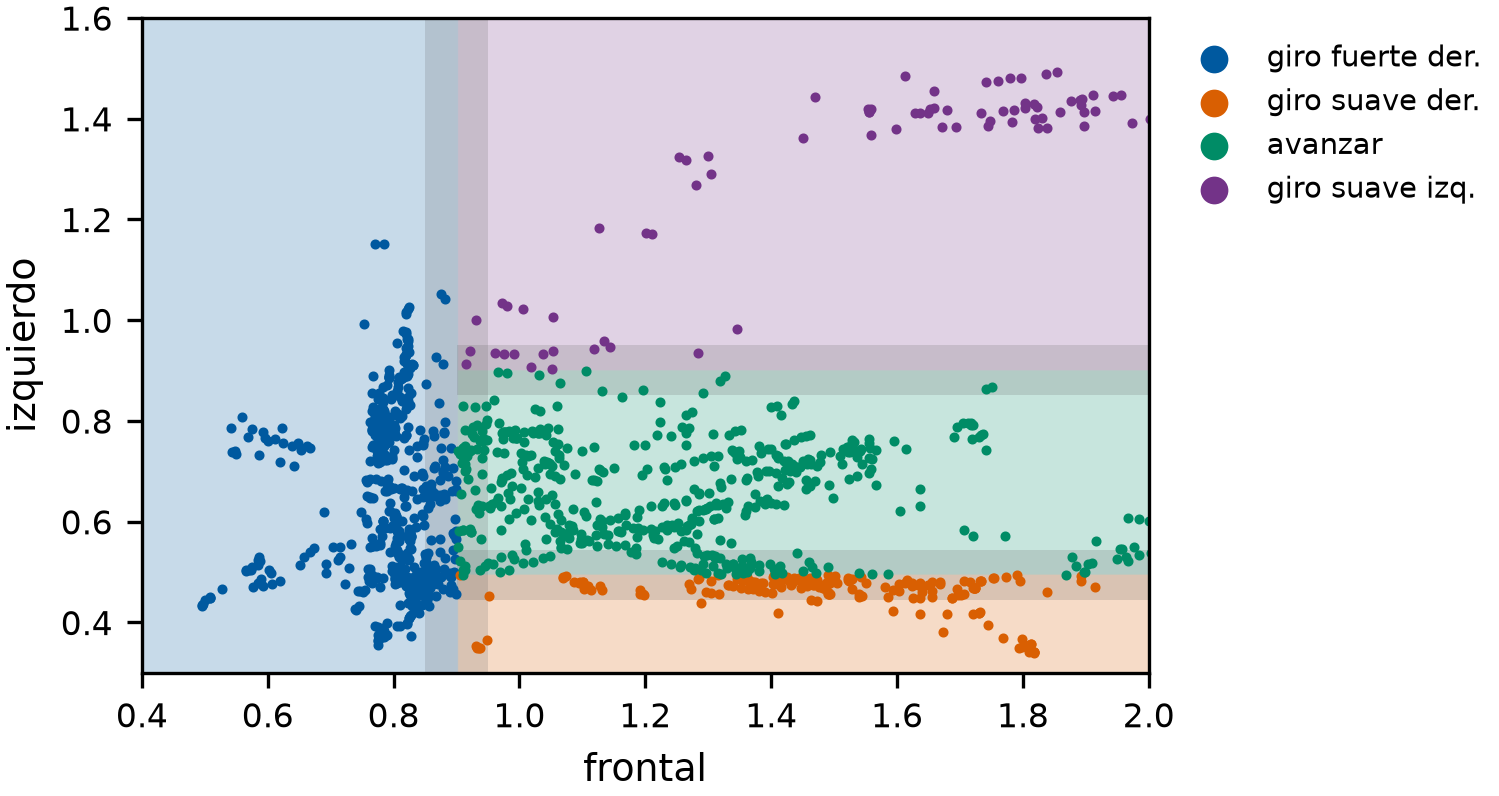
\includegraphics[width=12cm]{fig05_mapa.png}
    \caption{Acción que asigna el modelo de dos sensores en cada punto, con los registros de prueba encima. Las franjas grises son las transiciones entre acciones, de semiancho \semiancho{} alrededor de cada umbral. Quedan fuera de los ejes \fueraMapa{} registros de prueba}
    \label{fig:mapa}
\end{figure}

\subsection{Comparación con etiquetas uniformes}

La Tabla~\ref{tab:uniforme} y la Figura~\ref{fig:uniforme} muestran las cuatro variantes con etiquetas uniformes. El clasificador del cuaderno resuelto, con etiquetas entre el mínimo y el máximo y el consecuente del registro de mayor grado, llega a \uniCursoAcc~\% con dos sensores y $n=\uniCursoN$. En esa variante la acción avanzar solo acierta \uniCursoAvanzar{} de sus \nAvanzarTe{} registros de prueba. Con la suma de fuerzas y $n=\uniSumaN$ la exactitud sube a \uniSumaAcc~\%, aunque la balanceada baja. Con etiquetas en los cuantiles y el registro de mayor grado llega a \uniCuantAcc~\% con $n=\uniCuantN$ y \uniCuantReglas{} reglas. Con el mínimo y el máximo del entrenamiento, los límites de clase de la distancia izquierda, 0.495 y 0.900, quedan en \escIzqA{} y \escIzqB{} de la escala normalizada.

\begin{table}[!htb]
    \centering
    \caption{Variantes con etiquetas uniformes dentro del límite de 100 reglas, exactitudes en porcentaje. El número de etiquetas $n$ se eligió con la validación cruzada del entrenamiento. La rejilla es $n$ elevado al número de sensores. Con el registro de mayor grado se cuentan las reglas que aparecen en el entrenamiento, y con la suma de fuerzas toda la rejilla, incluidas las celdas sin soporte}
    \label{tab:uniforme}
    \scriptsize
    \setlength{\tabcolsep}{3.5pt}
    \begin{tabular}{c l l c S[table-format=3.0] S[table-format=3.0] S[table-format=2.1] S[table-format=2.1] S[table-format=2.1]}
        \toprule
        \textbf{Sensores} & \textbf{Escala} & \textbf{Consecuente} & {$n$} & {\textbf{Rejilla}} & {\textbf{Reglas}} & {\textbf{Validación}} & {\textbf{Prueba}} & {\textbf{Balanceada}} \\
        \midrule
\filasUniforme
        \bottomrule
    \end{tabular}
\end{table}

\begin{figure}[!htb]
    \centering
    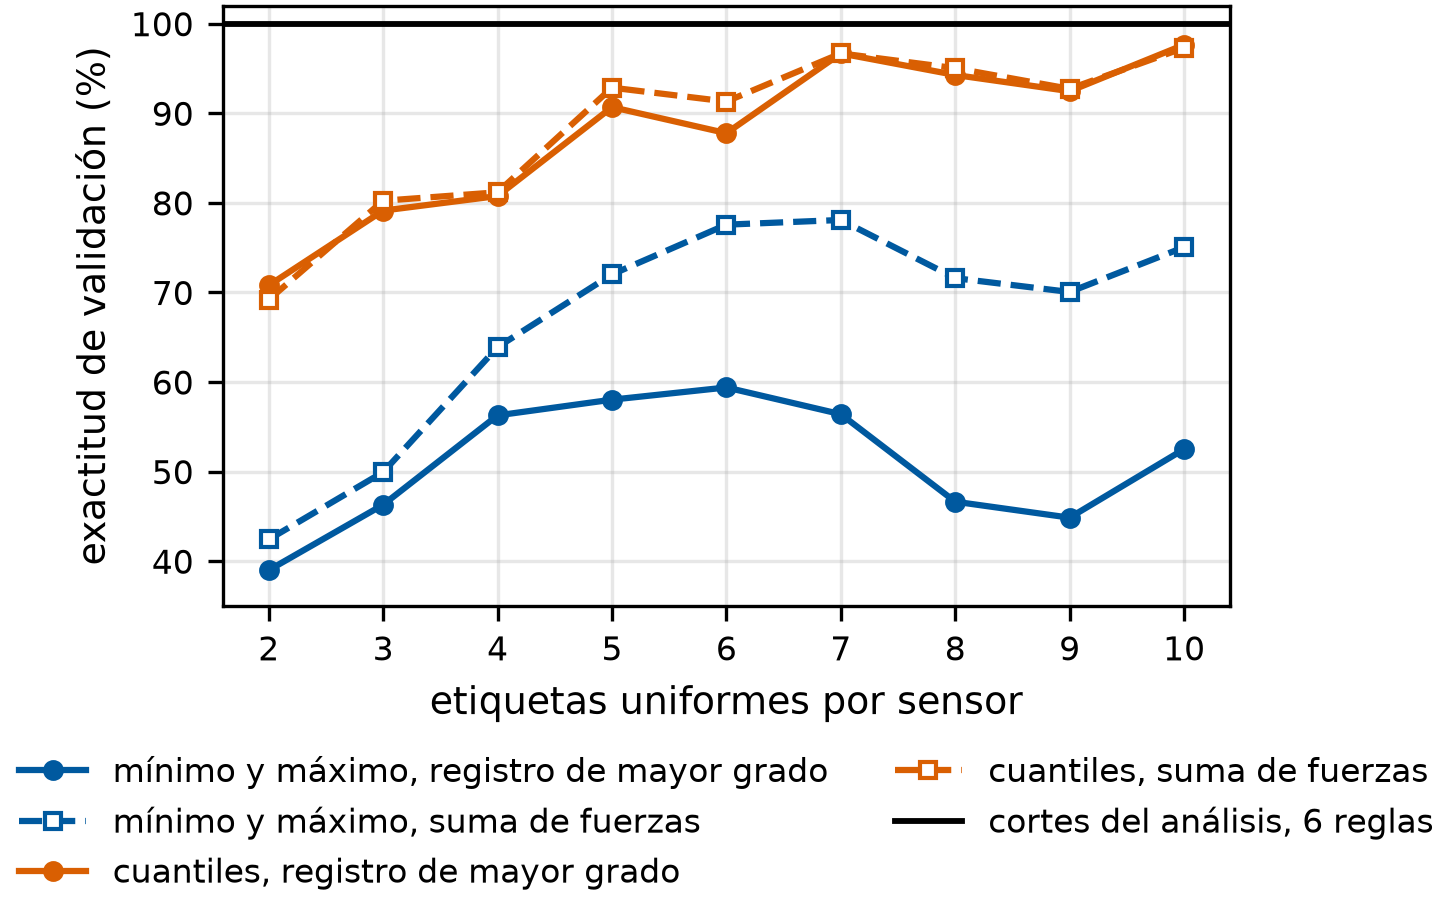
\includegraphics[width=14cm]{fig06_uniforme.png}
    \caption{Exactitud de validación cruzada en el entrenamiento de las cuatro variantes con etiquetas uniformes y dos sensores, frente al modelo con los cortes del análisis}
    \label{fig:uniforme}
\end{figure}

\subsection{Sensibilidad, ruido, salida continua y partición temporal}

La Figura~\ref{fig:sens} muestra la exactitud en prueba del modelo de dos sensores al mover cada umbral sin cambiar las reglas. Subir el umbral frontal 0.01 deja la exactitud en \sensFmas~\% y bajarlo 0.01 en \sensFmenos~\%, porque hay \cercaArriba{} registros de prueba justo por encima y \cercaAbajo{} justo por debajo. El umbral bajo de la izquierda da \sensBmas~\% al subirlo y \sensBmenos~\% al bajarlo, y el alto casi no importa, con un mínimo de \sensAmin~\% en todo el rango probado.

\begin{figure}[!htb]
    \centering
    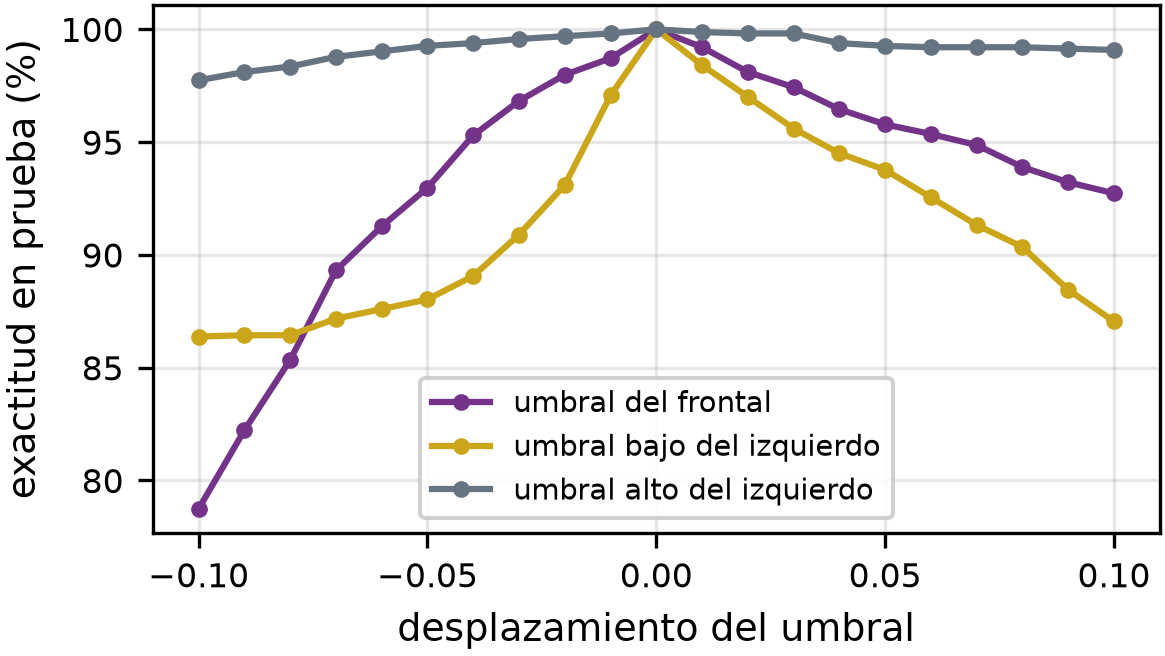
\includegraphics[width=11cm]{fig07_sensibilidad.png}
    \caption{Exactitud en prueba del modelo de dos sensores al desplazar un umbral y dejar los otros en su lugar}
    \label{fig:sens}
\end{figure}

La Tabla~\ref{tab:ancho} muestra que el semiancho de la transición no cambia la exactitud pero sí cuántos registros caen en una franja y la certeza de las reglas. Con $\delta=\semiancho$ el \dentroBanda~\% de los registros de prueba tiene una regla ganadora con fuerza menor que 1. En el \compite~\% hay además una regla activa de otra acción, y en el \misma~\% restante la que compite propone la misma acción. La Tabla~\ref{tab:ruido} agrega ruido gaussiano a las dos lecturas de prueba, con 20 realizaciones para cada desviación.

\begin{table}[!htb]
    \centering
    \caption{Efecto del semiancho de la transición en el modelo de dos sensores. La exactitud está en porcentaje, y la tercera columna es el porcentaje de registros de prueba cuya regla ganadora tiene fuerza menor que 1}
    \label{tab:ancho}
    \footnotesize
    \begin{tabular}{S[table-format=1.3] S[table-format=3.1] S[table-format=2.1] S[table-format=1.3]}
        \toprule
        {\textbf{Semiancho $\delta$}} & {\textbf{Exactitud en prueba}} & {\textbf{En una franja}} & {\textbf{Certeza mínima}} \\
        \midrule
\filasAncho
        \bottomrule
    \end{tabular}
\end{table}

\begin{table}[!htb]
    \centering
    \caption{Exactitud en prueba, en porcentaje, con ruido gaussiano en las lecturas frontal e izquierda. Media, mínimo y máximo de 20 realizaciones, y la menor fracción de predicciones iguales entre el modelo difuso y el árbol}
    \label{tab:ruido}
    \footnotesize
    \begin{tabular}{S[table-format=1.3] S[table-format=2.1] S[table-format=2.1] S[table-format=2.1] S[table-format=2.1] S[table-format=3.1]}
        \toprule
         & \multicolumn{3}{c}{\textbf{Difuso, 2 sensores}} & & \\
        \cmidrule(lr){2-4}
        {\textbf{Desviación}} & {\textbf{Media}} & {\textbf{Mínimo}} & {\textbf{Máximo}} & {\textbf{Árbol}} & {\textbf{Iguales}} \\
        \midrule
\filasRuido
        \bottomrule
    \end{tabular}
\end{table}

Usadas como Sugeno de orden cero, con giros de $-2$, $-1$, $0$ y $+1$ elegidos a mano en el orden del volante, las seis reglas dan un giro continuo (Figura~\ref{fig:sugeno}). En \nIntermedio{} registros de prueba el giro queda entre dos acciones. Al redondearlo a la acción más cercana la exactitud es \accSugeno~\%, y los \erroresSugeno{} registros que cambian están todos en la franja del umbral frontal. Allí el promedio entre el giro fuerte a la derecha y avanzar, o el giro suave a la izquierda, pasa por $-1$, y \erroresSuave{} de ellos se redondean a giro suave a la derecha, una acción distinta de la que propone la regla ganadora. La cifra depende de los giros elegidos, y con $-3$ para el giro fuerte sería \accSugenoB~\%.

Con la partición temporal los umbrales del frontal y del izquierdo salen iguales a los de la partición aleatoria, y los dos modelos aciertan todo el último 30~\% del recorrido. Los cortes de la derecha y la trasera sí cambian, de \uDerecho{} a \utDerecho{} y de \uTrasero{} a \utTrasero.

\begin{figure}[!htb]
    \centering
    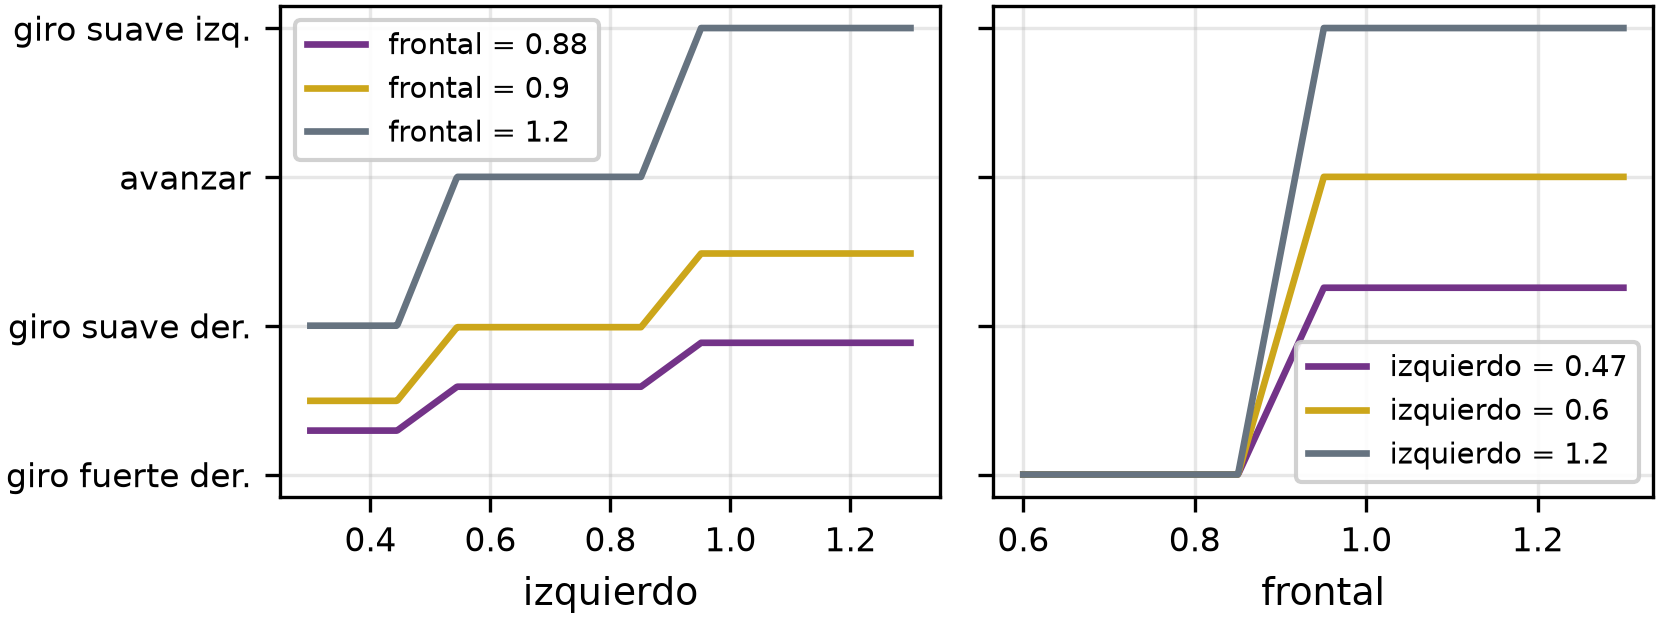
\includegraphics[width=14cm]{fig08_sugeno.png}
    \caption{Giro del Sugeno de orden cero con las seis reglas. Izquierda, en función de la distancia izquierda para tres lecturas frontales. Derecha, en función de la frontal para tres lecturas izquierdas}
    \label{fig:sugeno}
\end{figure}

\section{Análisis}

\subsection{De dónde sale el acierto completo}

Los rangos que no se tocan en la Tabla~\ref{tab:rangos} y la regla de tres umbrales que acierta los \aciertosNitida{} registros dicen lo mismo. En estos archivos la acción del robot es la salida de tres comparaciones, primero la distancia frontal contra \uFrontal{} y después la izquierda contra \uIzqBajo{} y \uIzqAlto. Eso concuerda con que las acciones las asignó un clasificador heurístico de reglas SI ENTONCES. Las reglas son las de un robot que recorre la sala en el sentido de las agujas del reloj, con la pared a su izquierda. Si hay un obstáculo cerca al frente gira fuerte a la derecha, si se acerca demasiado a la pared corrige un poco hacia la derecha, si se aleja corrige hacia la izquierda y en otro caso avanza. El acierto del 100~\% indica que el modelo difuso recupera el controlador que produjo las etiquetas. No dice cómo se comportaría el robot en otra sala, porque la prueba sale del mismo recorrido.

\subsection{Por qué fallan las etiquetas uniformes}

La Tabla~\ref{tab:uniforme} muestra que la causa principal es la escala. Las lecturas de la distancia izquierda tienen una cola larga, con valores aislados hasta 5.0, y entre el mínimo y el máximo del entrenamiento toda la zona que decide la acción queda comprimida al principio, con los límites de clase en \escIzqA{} y \escIzqB. Con $n$ triángulos uniformes la primera frontera entre etiquetas está en $1/(2(n-1))$, y para que llegue a \escIzqA{} harían falta unas \nNecesario{} etiquetas por sensor, \reglasNecesarias{} reglas con solo dos sensores. Con esa escala una sola celda junta acciones distintas. Con $n=\uniCursoN$ la celda que decide \avCelda{} de los \nAvanzarTe{} registros de avanzar de prueba reúne en el entrenamiento \mezclaAvanzar{} registros de avanzar y \mezclaSuave{} de giro suave a la derecha. El método del cuaderno toma la clase del único registro de mayor grado, que era de giro suave, y por eso avanzar acierta solo \uniCursoAvanzar{} veces. El consecuente no corrige la escala, solo decide qué acción pierde dentro de una celda mezclada. Con la suma de fuerzas las celdas mezcladas pasan a la acción mayoritaria, la exactitud sube a \uniSumaAcc~\% y la balanceada baja, porque las acciones minoritarias pierden aciertos. Las etiquetas en los cuantiles sí corrigen la escala y son la mejora más grande, de \uniCursoAcc{} a \uniCuantAcc~\%, y con dos sensores el registro de mayor grado queda incluso por encima de la suma de fuerzas. Aun así la mejor variante uniforme necesita \uniCuantReglas{} reglas para quedar en \uniCuantAcc~\%, mientras los histogramas por clase ponen las fronteras en los cambios de acción con seis.

\subsection{Cuatro sensores frente a dos}

Los dos modelos aciertan lo mismo en validación y en prueba, pero el de cuatro sensores necesita 24 reglas para expresar lo que el de dos dice con 6. Cada regla del segundo se reparte en cuatro según las etiquetas de las distancias derecha y trasera, que no cambian la decisión una vez conocidas la frontal y la izquierda. La trasera distingue en parte el giro suave a la izquierda, porque en esa acción suele ser mayor que en las demás (Tabla~\ref{tab:rangosdt}), pero la izquierda ya lo separa por completo. En 22 de las 24 reglas la acción aprendida coincide con la del modelo de dos sensores, y las \nDistintas{} que no coinciden tienen un soporte casi nulo. No ganan en prueba, pero un registro que cayera de lleno en una de ellas recibiría una acción equivocada. Ese riesgo crece con la rejilla, porque aparecen más celdas casi vacías. La elección entre los dos modelos se puede hacer sin mirar la prueba. El análisis de datos y la validación cruzada dicen que las distancias derecha y trasera sobran. El criterio visto en clase pide el modelo más simple cuya exactitud no se distinga de la del más complejo, y aplicado aquí a la validación del entrenamiento recomienda el modelo de dos sensores con seis reglas.

\subsection{Qué aporta lo difuso}

Con la regla más fuerte como decisión y trapecios que se cruzan en 0.5 justo en cada umbral, la frontera entre acciones es el umbral mismo. El modelo difuso decide entonces como el árbol de cuatro hojas, y la Tabla~\ref{tab:ruido} lo confirma, con predicciones idénticas a las del árbol para todos los niveles de ruido. Por la misma razón el semiancho $\delta$ no cambia ninguna predicción. Una fuerza ganadora menor que 1 indica cercanía a un corte y no siempre a un cambio de acción, porque en el \misma~\% de los registros la franja separa dos reglas con la misma acción. El cambio cercano lo indica una regla activa de otra acción, lo que ocurre en el \compite~\% de los registros con $\delta=\semiancho$. Las dos cosas se pueden calcular también con la distancia a los cortes del árbol. La certeza menor que 1 de la Tabla~\ref{tab:reglas} la produce $\delta$, porque las franjas hacen que registros de una acción activen en parte la regla vecina. Con $\delta=0.001$ la certeza mínima es 0.997.

Con una salida continua el resultado sí cambia. El Sugeno de orden cero de la Figura~\ref{fig:sugeno} cambia el giro de forma gradual dentro de cada franja en lugar de saltar de una acción a otra. Entre acciones vecinas, como en las franjas de la izquierda, el redondeo devuelve la acción nítida. Entre acciones no vecinas, como el giro fuerte a la derecha y avanzar en la franja frontal, el promedio pasa por una acción intermedia que la regla ganadora no propone, y de ahí salen los \erroresSugeno{} registros que bajan la exactitud a \accSugeno~\%. Promediar acciones solo tiene sentido cuando se ordenan en una escala, y aun así el resultado depende de los valores asignados a cada una.

\subsection{Sensibilidad y límites de la evaluación}

La Figura~\ref{fig:sens} mide sobre todo cuántos registros hay cerca de cada umbral. Un error de 0.01 en el umbral frontal cuesta 0.8 o 1.3 puntos según el sentido, porque hay \cercaArriba{} registros de prueba a menos de 0.01 por encima y \cercaAbajo{} por debajo. El umbral alto de la izquierda casi no importa porque pocos registros pasan cerca de 0.9 en esa distancia con el frente despejado. Fijar los umbrales con el punto medio entre clases del entrenamiento evita ese error, y con lecturas de resolución 0.001 y clases que no se tocan el punto medio queda determinado por los datos. El ruido de la Tabla~\ref{tab:ruido} mide cuánto se degrada la decisión si las lecturas que ve el modelo difieren de las que vio el controlador. Con una desviación de 0.01 en las dos lecturas la exactitud baja en promedio a \ruidoUno~\%, entre \ruidoUnoMin{} y \ruidoUnoMax~\% según la realización.

La partición temporal da el mismo resultado que la aleatoria. Las acciones siguen las mismas tres fronteras en todo el recorrido, y por eso el acierto no se debe a que la prueba tenga registros vecinos de los de entrenamiento. El último 30~\% del recorrido es la misma sala, así que tampoco esta partición prueba otro entorno.

\section{Conclusiones}

En la Tabla~\ref{tab:rangos} la distancia frontal separa el giro fuerte de las otras tres acciones, y con el frente despejado la izquierda separa esas tres sin que sus rangos se toquen. La regla nítida de tres cortes acierta los \aciertosNitida{} registros del archivo, así que la acción depende de la distancia frontal, con un corte en \uFrontal, y de la izquierda, con cortes en \uIzqBajo{} y \uIzqAlto. Por eso bastan dos etiquetas en la frontal y tres en la izquierda, cruzadas en esos cortes (Tabla~\ref{tab:mf}).

Con esas etiquetas el modelo de dos sensores tiene \reglasDos{} reglas y el de cuatro \reglasCuatro, y los dos aciertan los \nTe{} registros de prueba (Tablas~\ref{tab:resultados} y \ref{tab:confusion}). La partición temporal, que también acierta todo, descarta que el acierto venga de registros vecinos entre entrenamiento y prueba. Como las acciones las asignó un controlador de reglas nítidas, ese acierto indica que el modelo recupera el controlador, no cómo se comportaría el robot en otra sala.

Una vez conocidas la frontal y la izquierda, las distancias derecha y trasera no cambian ninguna decisión en prueba. En 22 de las 24 reglas del modelo de cuatro sensores la acción es la que dictan la frontal y la izquierda, y las dos que difieren tienen soportes de \distSoportes{} y no ganan en ningún registro de prueba (Tabla~\ref{tab:reglas4}). Por eso, y porque los dos modelos empatan en la validación del entrenamiento con \cvDos~\%, el modelo que se entrega como el mejor es el de dos sensores.

La ubicación de las etiquetas pesa más que su número. Con tres etiquetas por sensor en el modelo de cuatro, repartirlas por cuantiles en lugar de entre el mínimo y el máximo sube la prueba de \uniTresMinMax{} a \uniTresCuant~\% (Tabla~\ref{tab:uniforme}). Con dos sensores el clasificador del cuaderno resuelto llega a \uniCursoAcc~\%, y casi todo su error está en avanzar, que acierta \uniCursoAvanzar{} de \nAvanzarTe. Con los cortes de los histogramas por clase se llega al 100~\% con seis reglas (Tablas~\ref{tab:resultados} y \ref{tab:uniforme}). En Wine la partición uniforme había alcanzado 92.6~\%, y aquí deja de servir porque la cola larga de la distancia izquierda deja sus límites de clase en \escIzqA{} y \escIzqB{} de la escala.

En el taller propuesto el mínimo y el producto dieron las mismas predicciones, porque con la regla más fuerte gana la celda propia de cada registro. Aquí la forma de las etiquetas tampoco cambia la decisión. Con semianchos de 0.001 a 0.200 la exactitud sigue en 100~\% (Tabla~\ref{tab:ancho}), y con ruido en las lecturas el modelo difuso y el árbol de cuatro hojas, que corta en los mismos tres valores, dan las mismas predicciones en las 20 realizaciones de cada nivel (Tabla~\ref{tab:ruido}).

El margen entre clases en el entrenamiento es de una milésima, 0.900 frente a 0.901 en la frontal. Mover ese corte 0.01 cuesta entre 0.8 y 1.3 puntos, y un ruido de 0.01 en las lecturas baja la exactitud a \ruidoUno~\% en promedio (Figura~\ref{fig:sens} y Tabla~\ref{tab:ruido}). El modelo es exacto mientras las lecturas tengan la resolución con que se etiquetaron.

Como Sugeno de orden cero, las seis reglas dan un giro que cambia en rampa dentro de las franjas de $\pm$\semiancho, y al redondearlo la exactitud queda en \accSugeno~\%. Los \erroresSugeno{} registros que cambian están en la franja del corte frontal, donde se promedian acciones que no son vecinas (Figura~\ref{fig:sugeno}). La cifra depende de los giros elegidos, y con $-3$ para el giro fuerte sube a \accSugenoB~\%.

\section{Referencias}
\begin{itemize}
    \item Freire, A. L., Barreto, G. A., Veloso, M., \& Varela, A. T. (2009a). Short-term memory mechanisms in neural network learning of robot navigation tasks: A case study. \textit{6th Latin American Robotics Symposium (LARS)}, 1--6.
    \item Freire, A., Veloso, M., \& Barreto, G. (2009b). \textit{Wall-Following Robot Navigation Data}. UCI Machine Learning Repository. https://doi.org/10.24432/C57C8W
    \item Ishibuchi, H., Nozaki, K., \& Tanaka, H. (1992). Distributed representation of fuzzy rules and its application to pattern classification. \textit{Fuzzy Sets and Systems}, 52(1), 21--32.
    \item Ross, T. J. (2010). \textit{Fuzzy Logic with Engineering Applications} (3.ª ed.). Wiley.
    \item Takagi, T., \& Sugeno, M. (1985). Fuzzy identification of systems and its applications to modeling and control. \textit{IEEE Transactions on Systems, Man, and Cybernetics}, 15(1), 116--132.
    \item Wang, L.-X., \& Mendel, J. M. (1992). Generating fuzzy rules by learning from examples. \textit{IEEE Transactions on Systems, Man, and Cybernetics}, 22(6), 1414--1427.
    \item Zadeh, L. A. (1965). Fuzzy sets. \textit{Information and Control}, 8(3), 338--353.
\end{itemize}

\clearpage
\appendix
\section{Reglas del modelo de cuatro sensores}
\label{anexo:reglas}

\begin{table}[!htb]
    \centering
    \caption{Las 24 reglas del modelo de cuatro sensores, ordenadas por soporte en el entrenamiento. La última columna cuenta en cuántos registros de prueba ganó cada regla}
    \label{tab:reglas4}
    \scriptsize
    \setlength{\tabcolsep}{4pt}
    \begin{tabular}{c l l l l l S[table-format=3.1] S[table-format=1.3] S[table-format=3.0]}
        \toprule
        \textbf{Regla} & \textbf{Frontal} & \textbf{Izquierda} & \textbf{Derecha} & \textbf{Trasera} & \textbf{Acción} & {\textbf{Soporte}} & {\textbf{Certeza}} & {\textbf{Gana}} \\
        \midrule
\filasReglasCuatro
        \bottomrule
    \end{tabular}
\end{table}

\section{Código del diseño}

Se reproducen las funciones que construyen el modelo a partir del entrenamiento, tal como quedaron en el cuaderno.

\begin{lstlisting}[caption={Cortes y etiquetas desde las clases del entrenamiento}]
def corte(abajo, arriba):
    """Punto medio entre el mayor valor del grupo de abajo y el menor del grupo de arriba."""
    return float((np.max(abajo) + np.min(arriba)) / 2)

def corte_arbol(x, y):
    """Valor que mejor separa las clases con una sola variable (árbol de un nivel)."""
    return float(DecisionTreeClassifier(max_depth=1, random_state=SEMILLA).fit(x[:, None], y).tree_.threshold[0])

def disenar_mf(Xtr, ytr, delta=DELTA):
    """Umbrales y etiquetas a partir de las clases del entrenamiento."""
    f, i, de, t = Xtr.T
    libre = ytr != 0                                # frente despejado
    u = {"frontal": corte(f[ytr == 0], f[libre]),
         "izq_bajo": corte(i[ytr == 1], i[ytr == 2]),
         "izq_alto": corte(i[ytr == 2], i[ytr == 3]),
         "derecho": corte_arbol(de, ytr), "trasero": corte_arbol(t, ytr)}
    MF = {"frontal": dos_etiquetas(u["frontal"], delta=delta),
          "izquierdo": tres_etiquetas(u["izq_bajo"], u["izq_alto"], delta=delta),
          "derecho": dos_etiquetas(u["derecho"], delta=delta),
          "trasero": dos_etiquetas(u["trasero"], delta=delta)}
    return MF, u
\end{lstlisting}

\begin{lstlisting}[caption={Rejilla completa con consecuentes aprendidos}]
def crear_reglas(X, y, variables, MF, n_clases=4):
    """Rejilla completa. Consecuente = acción con mayor suma de fuerza; certeza = esa suma sobre el total."""
    R = np.array(list(itertools.product(*[range(len(MF[v])) for v in variables])))
    fuerza = fuerza_rejilla(grados(X, variables, MF), R)
    voto = np.stack([fuerza[y == c].sum(axis=0) for c in range(n_clases)], axis=1)
    soporte = voto.sum(axis=1)
    return R, voto.argmax(axis=1), soporte, voto.max(axis=1) / np.maximum(soporte, 1e-12)
\end{lstlisting}

\section{Archivos entregados}
\label{anexo:archivos}

El archivo ZIP de la entrega contiene este informe y una carpeta con todo lo necesario para repetir el experimento, cuyo nombre es \texttt{TallerRobot\_LogicaDifusa\_SergioDuarte}.

\begin{table}[!htb]
    \centering
    \caption{Contenido de la carpeta entregada}
    \label{tab:archivos}
    \footnotesize
    \begin{tabular}{>{\raggedright\arraybackslash}p{5.6cm} >{\raggedright\arraybackslash}p{9.4cm}}
        \toprule
        \textbf{Archivo} & \textbf{Contenido} \\
        \midrule
        \texttt{Taller\_LogicaDifusa\_Robot.ipynb} & Cuaderno completo y ejecutado con NumPy 2.4 y scikit-fuzzy 0.5, con el análisis, los dos modelos, las comparaciones y las dieciocho verificaciones \\
        \texttt{datos/sensor\_readings\_4.csv} & Distancias frontal, izquierda, derecha y trasera con la acción, como las entrega el aula \\
        \texttt{datos/sensor\_readings\_2.csv} & Distancias frontal e izquierda con la acción \\
        \texttt{particiones/aleatoria\_*.csv} & Grupos de entrenamiento (3\,819 registros) y de prueba (1\,637) de la partición aleatoria, para 4 y para 2 sensores, con el número de fila del archivo original \\
        \texttt{particiones/temporal\_*.csv} & Los mismos grupos para la partición temporal, primer 70~\% del recorrido y último 30~\% \\
        \texttt{modelos/modelo\_2\_sensores.json} & Modelo entregado como el mejor, con cortes, etiquetas, seis reglas, soporte y certeza \\
        \texttt{modelos/modelo\_4\_sensores.json} & Modelo de cuatro sensores con sus 24 reglas \\
        \texttt{resultados.json} & Cifras que usa este informe, escritas por el último paso del cuaderno \\
        \texttt{figuras\_informe.py} & Genera las figuras de este informe y sus cifras a partir de \texttt{resultados.json} \\
        \texttt{LEEME.txt} & Pasos para ejecutar el cuaderno y requisitos \\
        \bottomrule
    \end{tabular}
\end{table}

\end{document}
